% !TEX encoding = UTF-8
% !TEX TS-program = pdflatex
% !TEX root = ../tesi.tex

%**************************************************************
\chapter{Progettazione e codifica}
\label{cap:progettazione-codifica}
%**************************************************************

La seguente sezione ha lo scopo di illustrare la soluzione ideata dal laureando per il soddisfacimento dei requisiti concordati con il tutor aziendale descritti nel capitolo \ref{cap:descrizione-stage}. In ciascuna sezione viene presentata una maschera dell'applicativo sviluppata, con il dovuto corredo di immagini e \gls{snippets} di codice.


\section{L'applicativo SyncRec: Struttura e sviluppo del progetto}

\begin{figure}[!h] 
	\centering 
	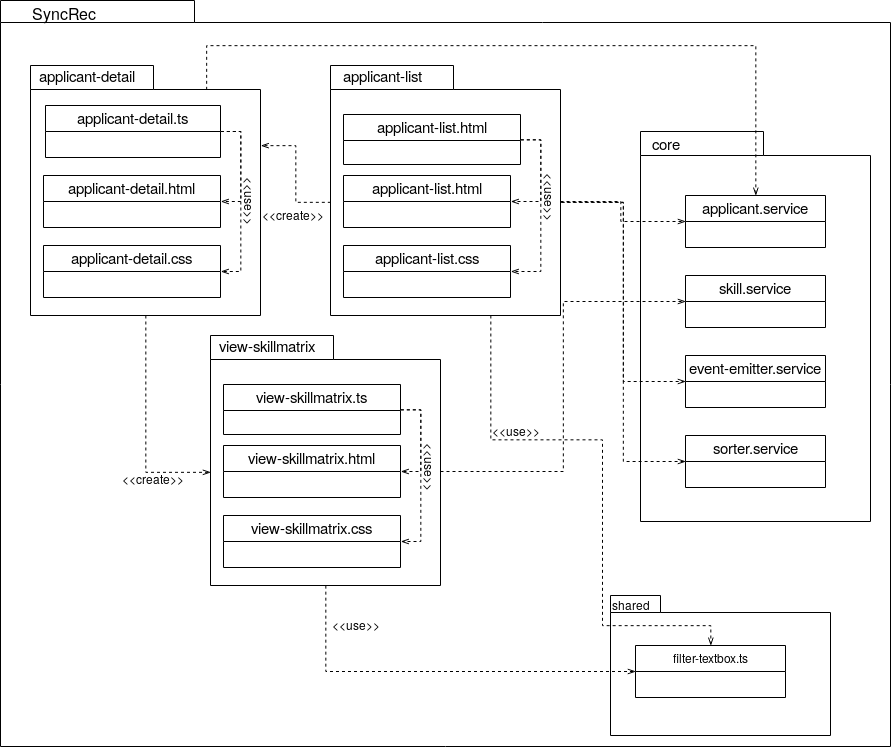
\includegraphics[width=1\columnwidth]{immagini/usecase/UML1} 
	\caption{Struttura dei \textit{component} sviluppati per l'applicativo SyncRec}
	\label{figura:UML1}
\end{figure}

Come già accennato in precedenza, \hyperref[angular]{Angular} suggerisce di applicare una forte struttura modulare alle proprie \gls{web application}, tale approccio è stato nella gran parte perseguito, con alcune eccezioni per determinati elementi condivisi fra più \textit{component}; un'applicazione di tale struttura, inoltre, permette lo sviluppo delle proprie componenti senza dover necessariamente conoscere l'intera architettura nel dettaglio.

La figura \ref{figura:UML1} illustra la struttura dei \textit{component} sviluppati per l'applicativo SyncRec, a scopo di sintesi sono state omesse alcune parti proprie del \gls{framework} di riferimento (come i moduli e gli \textit{asset}) o sviluppate da altri studenti nel corso del progetto.\\
I moduli \textit{applicant-list}, \textit{applicant-detail} e \textit{viewskillmatrix} rappresentano i componenti grafici dell'applicazione, il modulo \textit{shared} rappresenta l'insieme di \textit{component} condivisi nel \textit{namespace} globale e il modulo \textit{core} contiene i \textit{service}; quest'ultimi hanno il duplice scopo di recuperare i dati dal \gls{Back-end} e di fornire alcuni metodi di utilità necessari a svolgere determinate operazioni (come l'ordinamento o l'emissione di eventi verso \textit{components} padri).\\
La figura \ref{figura:UML2} illustra come il modulo \textit{service} si occupi di dialogare con il \gls{Back-end} scritto in \hyperref[tech-spring]{Spring}.\\
In ambito di progettazione, dialogando con gli altri laureandi che hanno preso parte alla realizzazion di SyncRec, si sono definite alcune linee guida da perseguire nel corso della codifica.\\
Tali linee guida sono:
\begin{itemize}
	\item Utilizzare il più possibile le direttive \hyperref[angular]{Angular} (come \gls{ng-Model}) all'interno del \textit{HTML} dei \textit{component}.
	\item Definire per ciascun \textit{component} il relativo modulo di referimento, tale prassi è fortemente consigliata dalla documentazione di \hyperref[angular]{Angular}.
	\item Per quanto riguarda il \textit{CSS}, favorire l'utilizzo della versione 3.0 piuttosto che della libreria esterna \textit{bootstrap}.
\end{itemize}

\begin{figure}[!h] 
	\centering 
	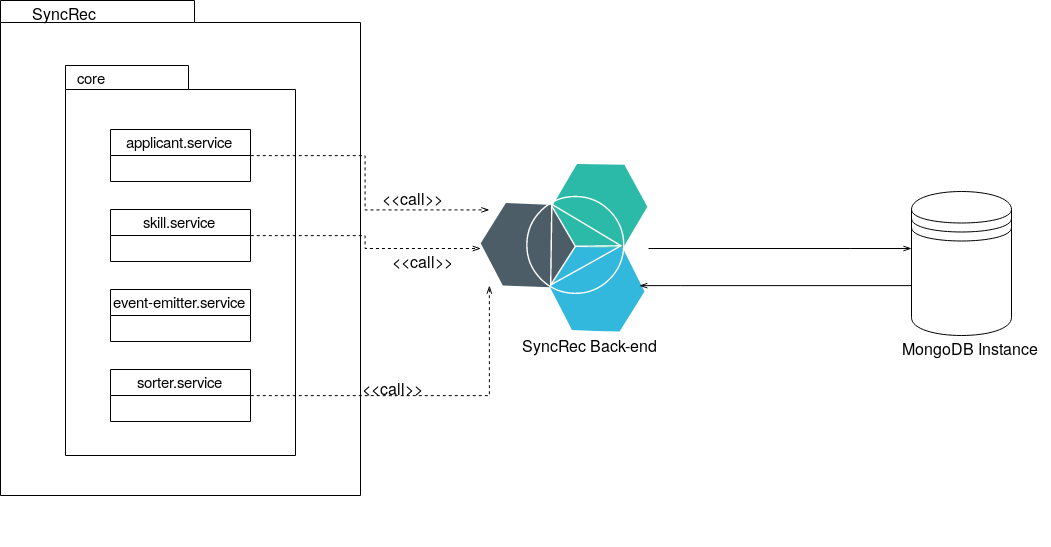
\includegraphics[width=1\columnwidth]{immagini/usecase/UML2} 
	\caption{Integrazione tra Front-end e Back-end}
	\label{figura:UML2}
\end{figure}

\subsection{Homepage}
La homepage dell'applicativo (v. figura \ref{figura:homepage}) si presenta come un semplice menù con 3 voci.
\begin{itemize}
	\item \textbf{Aggiungi persone} reindirizza verso il \textit{component} adibito all'aggiunta degli \textit{applicant};
	\item \textbf{Visualizza persone} reindirizza verso il \textit{component} adibito alla visualizzazione della lista degli \textit{applicant}, sviluppato dal laureando nel corso del progetto di stage;
	\item \textbf{Ricerca Persone} reindirizza verso il \textit{component} adibito alla ricerca delle persone;
\end{itemize}
In aggiunta, è possibile effettuare il \textit{logout} con un pulsante posto in alto, vicino al logo.
\vspace{0.5em}
\begin{figure}[!h] 
	\centering 
	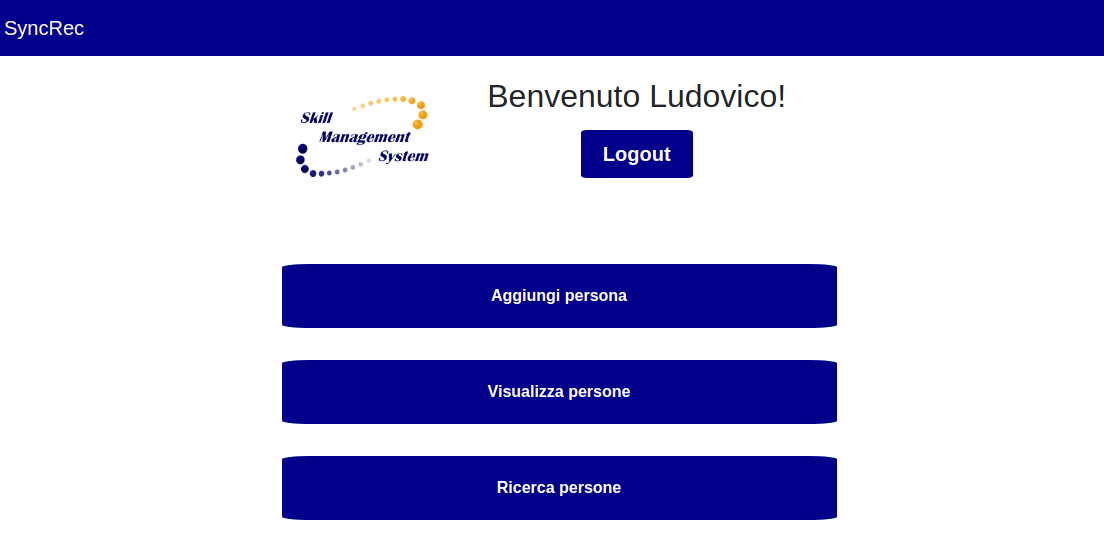
\includegraphics[width=1\columnwidth]{immagini/svil/homepage} 
	\caption{Schermata della homepage}
	\label{figura:homepage}
\end{figure}

\subsection{Maschera della visualizzazione degli\applicant} \label{section: applicant-list}
La fugura \ref{figura:lista}, mostra il \textit{component} sviluppato per la visualizzazione degli \textit{applicant}, per ciascun \textit{applicant} viene visualizzato il Cognome, il Nome e l'email, insieme a un tasto per l'eliminazione e uno per la visualizzazione del dettaglio della persona, il quale reindirizza verso la maschera descritta nella sezione \ref{m-CRUD}.\\
Per realizzare questa \textit{task}, è stato necessario reperire le informazione tramite un \textit{service} definito appositamente, il quale effettua una semplice \textit{GET} al relativo microservizio sviluppato nel \gls{Back-end} (v. codice \ref{get-applicant}).
Successivamente, i dati vengono memorizzati in un apposito \textit{array} e visualizzati tramite una direttiva \hyperref[angular]{Angular} chiamata \textit{ng-for} (v. \textit{listing}  \ref{ng-for}).

\vspace{0.5em}
\begin{figure}[!h] 
	\centering 
	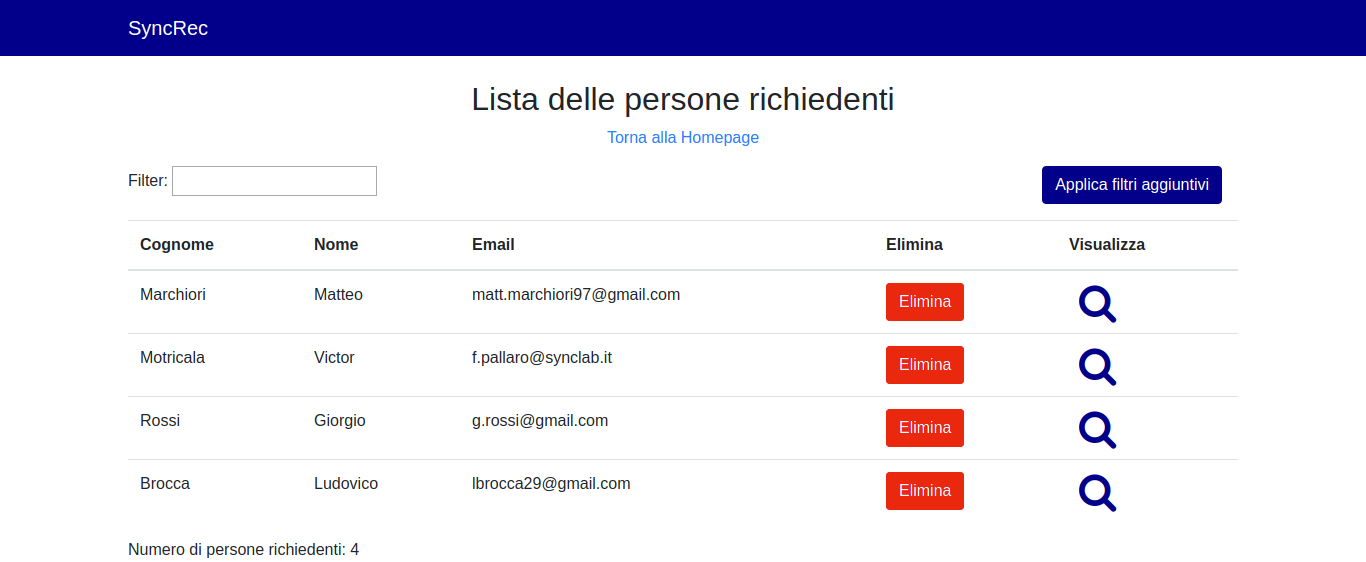
\includegraphics[width=1\columnwidth]{immagini/svil/lista} 
	\caption{Schermata della visualizzazione lista degli \textit{applicant}}
	\label{figura:lista}
\end{figure}

\begin{lstlisting}[label=get-applicant,caption=Funzione del service che effettua la chiamata GET]
getAllApplicants(): Observable<Applicant[]> {
	return this.http.get<Applicant[]>(this.baseUrl).pipe(
		catchError(this.handleError)
	);
}
\end{lstlisting} 

\begin{lstlisting}[label=ng-for,caption=Visualizzazione degli applicant nel codice HTML]
<tr class="hover-tr" *ngFor="let appl of filteredApplicants;" >
	<td>
		{{ appl.surname }}
	</td>
	<td>
		{{ appl.name }}
	</td>
	<td>
		{{ appl.email }}
	</td>
	<td>
	<button class="btn" id="btn-delete-applicant-list"
		(click)="deleteApplicant(appl.id)">Elimina</button>
	</td>
	<td>
	<span class="immagineEsterna" (click)="routerRedirect(appl.id)"><i class="fa fa-search fa-2x"></i></span>
	</td>
</tr>
\end{lstlisting} 

Il pulsante posto in alto a destra visualizza il \textit{component} adibito all'applicazione di filtri aggiuntivi sul totale degli \textit{applicant}, come si può vedere in figura \ref{figura:filtri}.\\
Posti sopra la tabella, inoltre, è possibile visualizzare un campo di testo, che permette di filtrare i risultati secondo nome, cognome o email. Tale filtro dinamico è stato ottenuto tramite l'azione congiunta di un \textit{service} (v \textit{listing}. \ref{event-e}) e di un \textit{component} costituito da un singolo campo di testo; il \textit{component} padre in questo modo può applicare il filtro sugli \textit{applicant} ogni qualvolta il contenuto del campo di testo venga cambiato (v \textit{listing} \ref{filter}), in modo simile a quanto accade con l'\gls{Observer Pattern}.

\begin{lstlisting} [label=event-e, caption= Event-Emitter service]
export class EventEmitterService {

	invokeFirstComponentFunction = new EventEmitter();
	// variabile per la sottoscrizione di un component per la // reazione  ad eventi lanciati
	subsVar: Subscription;

	constructor() { }

	onComponentAction() {
		this.invokeFirstComponentFunction.emit();
	}
}
\end{lstlisting}

\begin{lstlisting} [label=filter, caption= Funzione che filtra i dati degli applicant]
filter(data: string) {
	if (data) {
		this.filteredApplicants = this._applicants.filter((applicant: Applicant) => {
			return applicant.name.toLowerCase().indexOf(data.toLowerCase()) > -1 ||
			applicant.surname.toLowerCase().indexOf(data.toLowerCase()) > -1 ||
			applicant.email.toLowerCase().indexOf(data.toLowerCase()) > -1;
		});
		} else {
		this.filteredApplicants = this._applicants;
	}
}

\end{lstlisting}

La visualizzazione del \textit{component} relativo all'aggiunta di filtri aggiuntivi viene gestita tramite una semplice direttiva \hyperref[angular]{Angular} chiamata \textit{Ng-if}, la quale si lega a una variabile booleana e determina la visualizzazione o meno del \textit{component} a seconda del valore assegnato. La selezione dei valori, invece, viene gestita tramite i \textit{form} \hyperref[angular]{Angular}, i quali legano i valori contenuti nei vari \textit{widget} a delle strutture che gestiscono autonomamente valori di default, validazione, \textit{submit} dei risultati e quant'altro, rendendo la struttura molto solida, sicura e poco soggetta a errori.
Nel \textit{listing} \ref{form} è possibile vedere l'inizializzazione del \textit{FormBuilder}, la sopracitata struttura in grado di gestire i dati di un \textit{form}, notare che viene inserito un pattern per la validazione ove necessario.
\newpage
\begin{lstlisting}[label= form, caption= Inizializzazione di un FormBuilder]


this.filterGroup = this.formBuilder.group({
	sesso: [''],
	name: ['',  Validators.pattern('^[a-zA-Z]*$')],
	surname: ['',  Validators.pattern('^[a-zA-Z]*$')],
	qualification: [''],
	seniority: [''],
	ambito: [''],
	geodisp: this.formBuilder.array([]),
	skill: [''],
	skillLevel: [''],
	scartato: [false],
});

\end{lstlisting}

\vspace{0.5em}
\begin{figure}[!h] 
	\centering 
	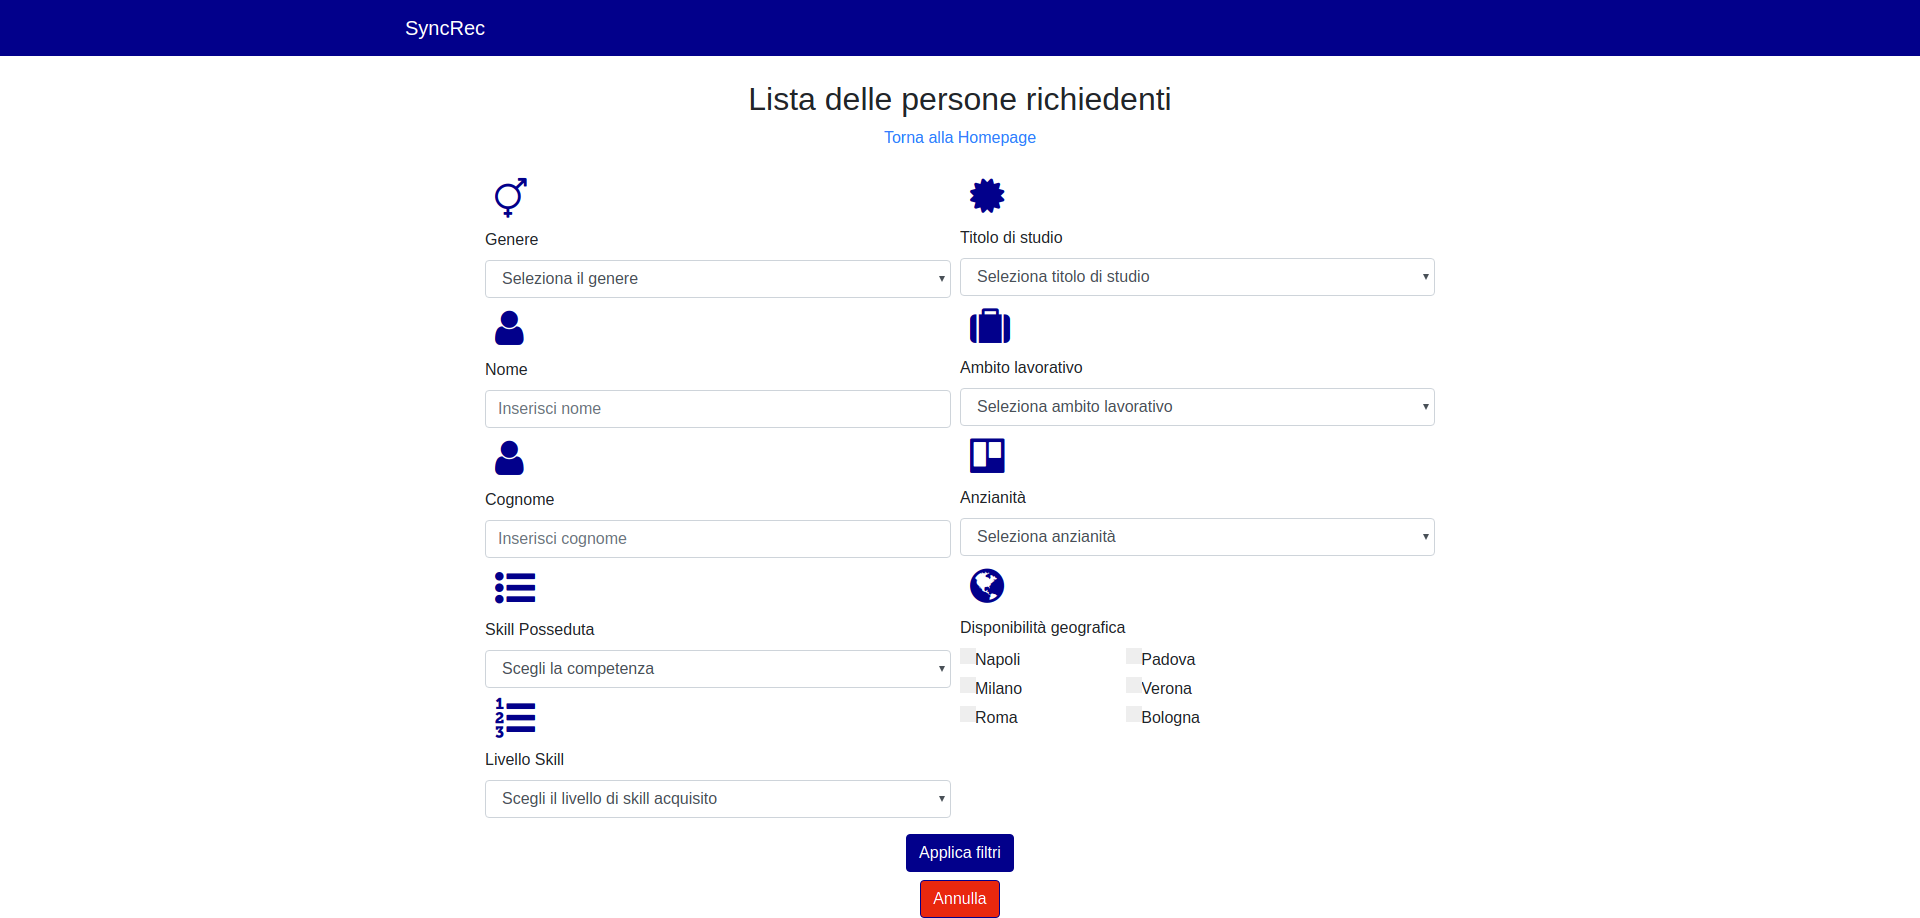
\includegraphics[width=1\columnwidth]{immagini/svil/filtri} 
	\caption{Schermata della selezione dei filtri da applicare alla lista degli \textit{applicant}}
	\label{figura:filtri}
\end{figure}

\subsection{Maschera delle operazioni CRUD su un\applicant}\label{m-CRUD}
\vspace{0.5em}
\begin{figure}[!h] 
	\centering 
	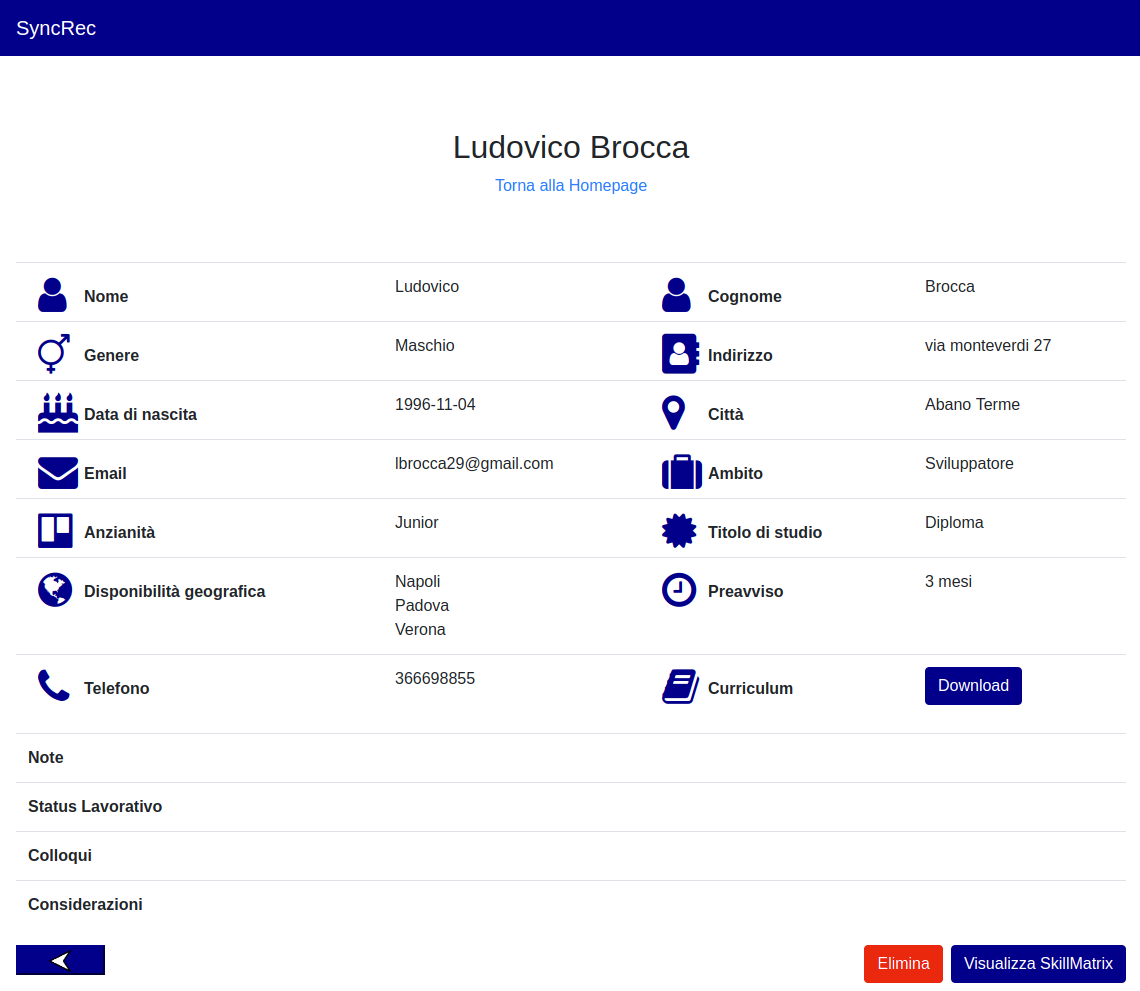
\includegraphics[width=1\columnwidth]{immagini/svil/applicant}
	\caption{Maschera \gls{CRUD} del singolo \textit{applicant}}
	\label{figura:applicant}
\end{figure}
La gestione delle operazioni \gls{CRUD} di un \textit{applicant} avviene tramite la maschera visible nella figura \ref{figura:applicant}; l'approccio adottato è molto simile a quanto avviene con la gestione della maschera per la selezione dei filtri aggiuntivi descritta nella sezione \ref{section: applicant-list}. Viene utilizzato un \textit{FormBuilder} per la gestione dei singoli valori di un \textit{applicant}, una volta modificati, un controllo su un parametro dei \textit{FormControl}, chiamato \texttt{touched}, permette la visualizzazione dei tasti di conferma o annullamento delle modifiche, in caso di conferma viene effettuata una chiamata \textit{PUT} tramite l'apposito servizio (descritta nel \textit{listing} \ref{PUT-call}), in caso contrario vengono ripristinati i valori antecedenti alle modifiche apportate dall'utente.\\
\newpage
\begin{lstlisting}[label=PUT-call, caption=chiamata PUT al microservizio del Back-end di SyncRec]
putApplicant(applicant: Applicant): Observable<any> {
	return this.http.patch(this.baseUrl + '/' + applicant.id, applicant).pipe(
		catchError((err: HttpErrorResponse) => {
			if (err.error instanceof Error) {
				// A client-side or network error occurred.
				const details = {detail: err.error, status: err.status};
				return throwError(details);
			} else {
				// The backend returned an unsuccessful response code.
				const details = {detail: err.error, status: err.status};
				return throwError(details);
			}
		})
	);
	
}
\end{lstlisting}
Con i pulsanti posti in basso è possibile tornare indietro, eliminare un \textit{applicant} (tramite una chiamata DELETE al microservizio di \gls{Back-end}), o visualizzare l'insieme di competenze possedute tramite l'apposita maschera descritta nella sezione \ref{section:skillmatrix}
\vspace{0.5em}.

\subsection{Maschera di visualizzazione di uno skillmatrix}\label{section:skillmatrix}
\begin{figure}[!h] 
	\centering 
	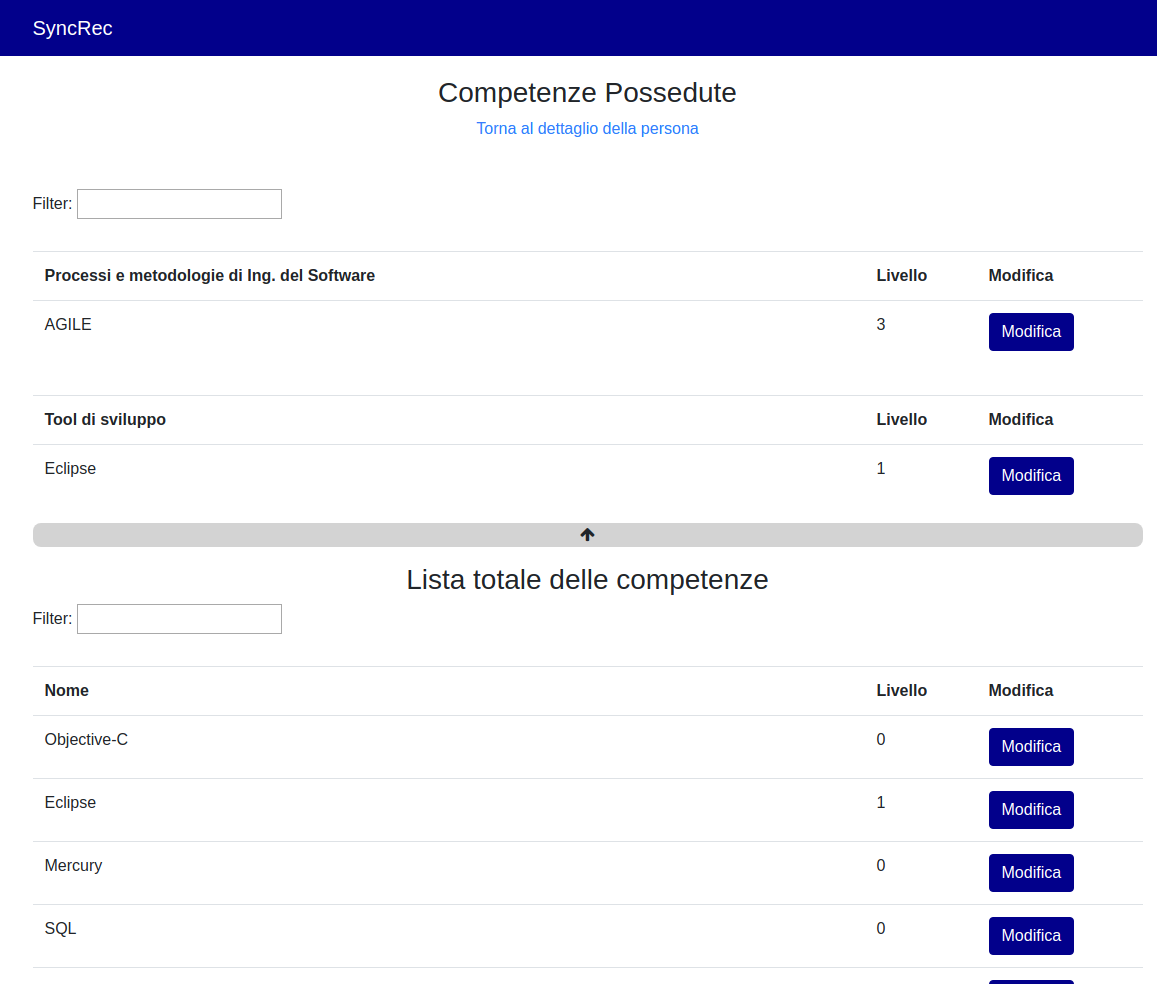
\includegraphics[width=1\columnwidth]{immagini/svil/skillmatrix} 
	\caption{Maschera CRUD dello skillmatrix}
	\label{figura:skillmatrix}
\end{figure}
Uno \textit{skillmatrix} rappresenta l'insieme delle competenze possedute da un \textit{applicant} insieme al relativo livello, che può variare da 0 a 5; una competenza per essere considerata posseduta deve avere un livello $\geq  5$.\\
\'E importante evidenziare come all'interno di SyncLab le competenze prese in considerazione siano molto numerose e tra le più disparate: nel contesto del progetto esse sono suddivise in categorie e il loro numero complessivo supera 130; ciò ha richiesto la formulazione di una soluzione che rendesse immediatamente visibile il distacco fra \textit{skill} possedute o meno e che al contempo  permettesse di modificare i valori in modo rapido.\\
Come si può vedere nella figura \ref{figura:skillmatrix}, l'approccio adottato prevede la predisposizione di 2 tabelle, una immediatamente visibile contenente l'insieme di \textit{skill} possedute per ciascuna categoria e una visibile tramite la pressione di un tasto, contenente il totale delle \textit{skill} considerate.\\
La visualizzazione delle skill è legata alla funzione \ref{categ}, che restiuisce un booleano a una direttiva \textit{Ng-If} all'interno del codice \textit{HTML}; la quale determina la visualizzazione o meno del codice afferente al \textit{tag} legato alla direttiva, come si può vedere nel \textit{listing} \ref{skVis}.\\
\newpage
\begin{lstlisting}[label=categ, caption=Funzione che determina la visualizzazione di una categoria avente \textit{skills} possedute ]

hasThisCategorySkills(cat: string): boolean {
	let result = false;
	const category: Category = this.catalog.filter ((c: Category) => c.name === cat)[0];
	category.skills.forEach((categoryskill) => {
		this.skills.filter((sk: Skill) => {
			if (categoryskill.name === sk.name && sk.level > 0) {
				result = true;
			}
		});
	});
	return result;
}

\end{lstlisting}

Per facilitare la navigazione fra le due tabelle, viene aggiunto il \textit{component} per il filtraggio dei dati, adottando lo stesso approccio della maschera di visualizzazione lista degli \textit{applicant} (v. sez. \ref{section: applicant-list}).\\
La modifica avviene tramite un menù a tendina visibile tramite la pressione di un tasto "Modfica", la tabella di \textit{skill} possedute si aggiorna in conseguenza alla conferma del nuovo dato selezionato (aggiungendo o togliendo righe a seconda del livello della \textit{skill}).\\
Allo scopo di rendere i dati consistenti fra le due tabelle (in modo da evitare che i livelli risultino discordanti), viene utilizzato un singolo \textit{FormBuilder} e una singola struttura dati che tenga traccia dei valori per il \textit{submit} delle modifiche.\\
 
 
 \begin{lstlisting} [label=skVis, caption= HTML e direttiva Ng-If]
 <ng-container *ngIf="hasThisCategorySkills(catalog[0].name)">
 <!-- direttiva che lega al FormBuilder del component -->
 <form [formGroup]="skillGroup">
 <!-- visualizzazione HTML di una tabella -->
 </form>
 </ng-container>
 \end{lstlisting}
   